
%(BEGIN_QUESTION)
% Copyright 2015, Tony R. Kuphaldt, released under the Creative Commons Attribution License (v 1.0)
% This means you may do almost anything with this work of mine, so long as you give me proper credit

Suppose a DP transmitter is connected to a process vessel so it may measure a vacuum inside that vessel.  Calculate the amount of differential pressure ``seen'' by this electronic DP transmitter in units of PSID, then calculate its output signal assuming a calibrated range of 0 to 380 inches water column differential and an output range of 4-20 mA:

$$\includegraphics[width=15.5cm]{i03939x01.eps}$$

There is definitely more than one way to calculate the transmitter's output signal value!  Outline more than one of these solutions.

\vskip 10pt

Furthermore, suppose an instrument technician decides to remove this transmitter from service in order to disconnect it from the process and then calibrate it back at the instrument shop.  Describe how the technician should operate the block and bleed valves to safely remove it from service, and then describe what the technician should do {\it before} operating either the block or the bleed valve to ensure no process upsets occur as a result.

\vskip 20pt \vbox{\hrule \hbox{\strut \vrule{} {\bf Suggestions for Socratic discussion} \vrule} \hrule}

\begin{itemize}
\item{} What safety hazards might there be for a technician disconnecting and connecting a pressure transmitter to a process vessel such as this?
\item{} Demonstrate how to {\it estimate} numerical answers for this problem without using a calculator.
\item{} What might happen if the vent tube on the ``L'' side of the transmitter were to become completely plugged?
\end{itemize}

\underbar{file i03939}
%(END_QUESTION)





%(BEGIN_ANSWER)

\noindent
{\bf Partial answer:}

\vskip 10pt

Applied differential pressure = +12.26 PSID

\vskip 10pt

Transmitter output signal = 18.29 mA

\vskip 10pt

Prior to operating either the block or the bleed valve, the technician should first notify operations personnel that the transmitter will be taken out of service and therefore will {\it not} register any process vacuum in the near future.  If the transmitter connects to a controller, that controller will need to be placed into manual mode.  If the transmitter connects to any pressure alarms or (worse yet!) an emergency shutdown system, those alarms will have to be disabled and/or the shutdown function will have to be bypassed before taking the transmitter out of service.

%(END_ANSWER)





%(BEGIN_NOTES)

$P_{high}$ = 748 mmHgA = 0.9842 Atm = 14.468 PSIA 

$P_{low}$ = 0.15 Atm = 2.205 PSIA

$\Delta P$ = 14.468 PSIA $-$ 2.205 PSIA = 12.263 PSID

\vskip 10pt

Shut the block valve first, then open the bleed valve in order to remove the transmitter from service.

\vskip 10pt

Incidentally, the atmospheric pressure of 748 torr is equivalent to an altitude of 136 meters above sea level, which makes this a very realistic figure for an industrial application.

%INDEX% Physics, units and conversions: pressure

%(END_NOTES)


